\section{Experiments}
In this section, we report our reproduction effort and verification of the experimental results in the paper.

\subsection{Toy Example}

We first reproduced the toy example about 1D Gaussian mixture mentioned in the paper. The task is to use SVGD to approximate a target distribution with PDF $p(x) = \frac{1}{3} N(x; -2, 1) + \frac{1}{3} N(x; 2, 1)$. The particles are initialized by an i.i.d. sample from the distribution $N(-10, 1)$, which is far away from the mode of the target distribution. We use 100 particles and 500 iterations with step size 0.25. 

As shown in figure \ref{fig:toy1dgaussian}, SVGD effectively recovered the distribution.


\begin{figure}[h]
    \centering
    \begin{tabular}{@{}c@{}}
        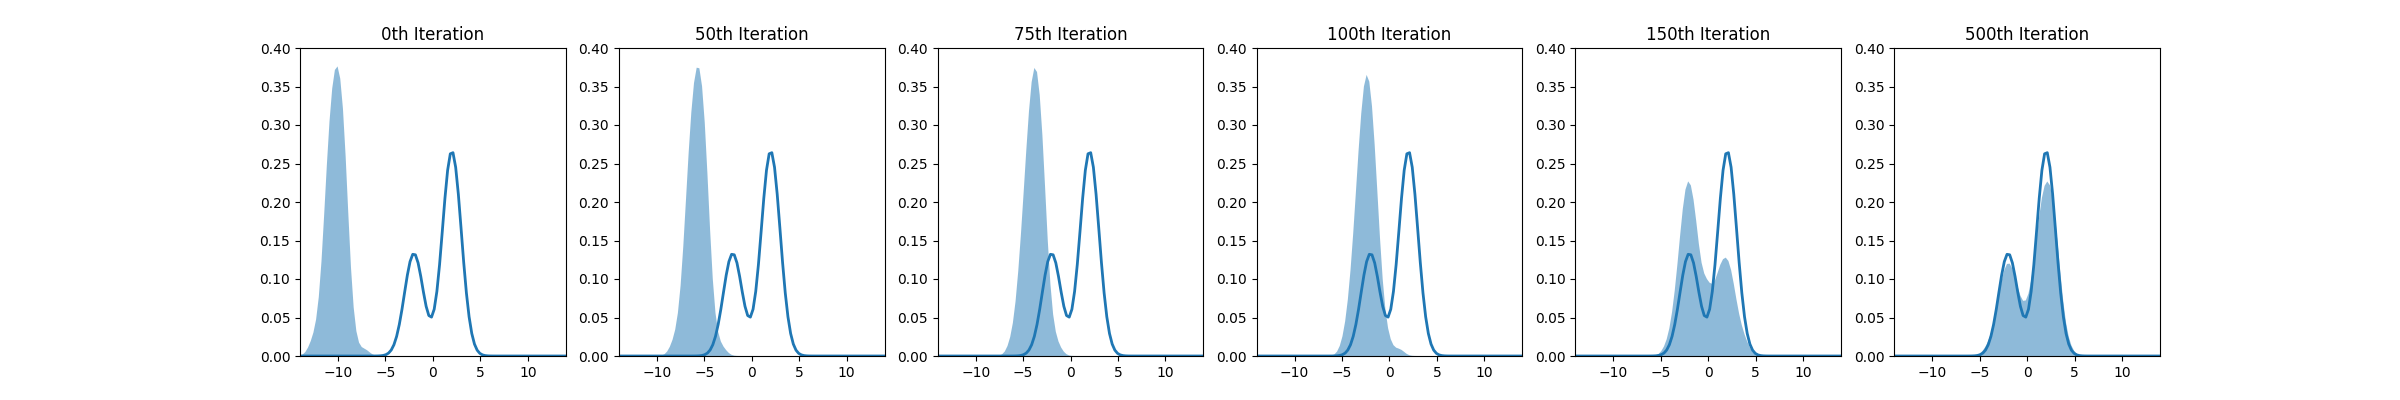
\includegraphics[width=\textwidth]{figs/toy-figure1_step0.1_mu2.0_w0.33_gaussian.png} \\
        \small (1) StepSize = 0.1, $\mu = \pm 2$, $(w_1, w_2) = (0.33, 0.67)$
    \end{tabular}
    
    \begin{tabular}{@{}c@{}}
        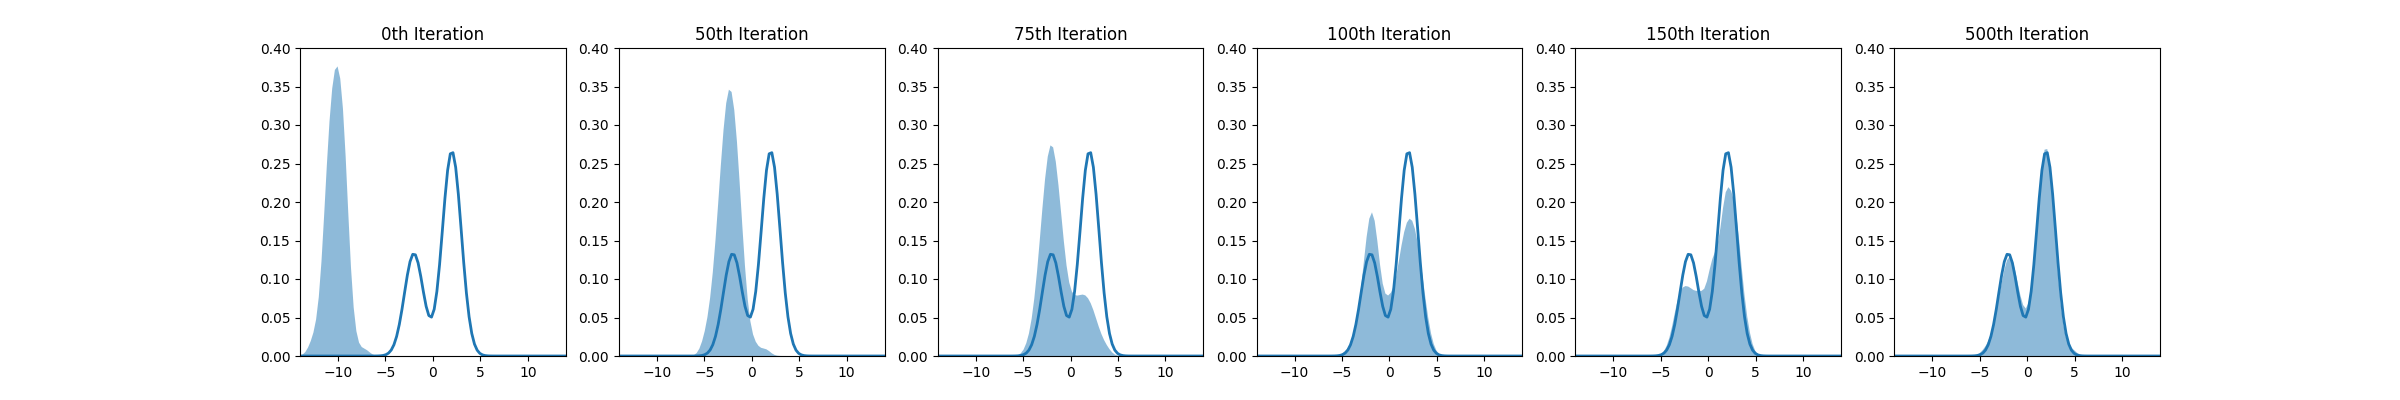
\includegraphics[width=\textwidth]{figs/toy-figure1.png} \\
        \small (2) StepSize = 0.25, $\mu = \pm 2$, $(w_1, w_2) = (0.33, 0.67)$
    \end{tabular}
    %\vspace{\floatsep}
    
    \begin{tabular}{@{}c@{}}
        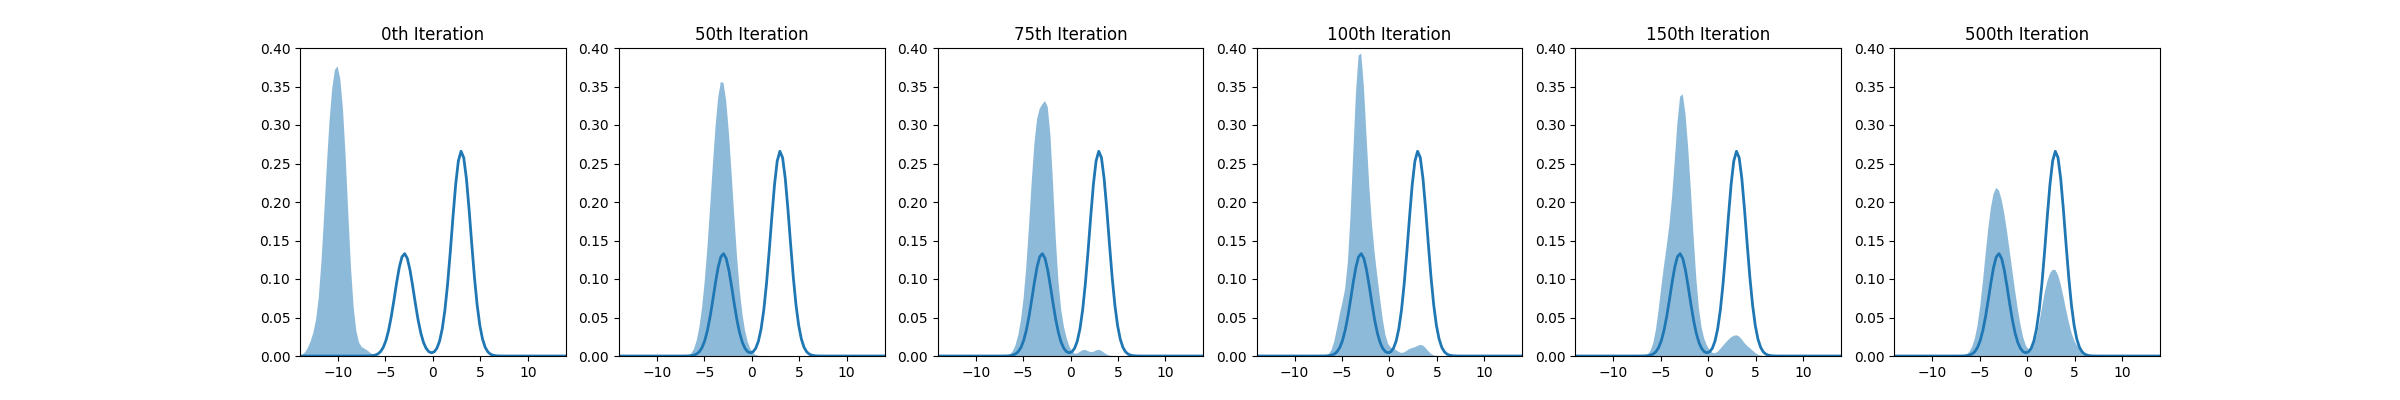
\includegraphics[width=\textwidth]{figs/toy-figure1_step0.25_mu3.0_w0.33_gaussian.png} \\
        \small (3) StepSize = 0.25, $\mu = \pm 3$, $(w_1, w_2) = (0.33, 0.67)$
    \end{tabular}
    
    \begin{tabular}{@{}c@{}}
        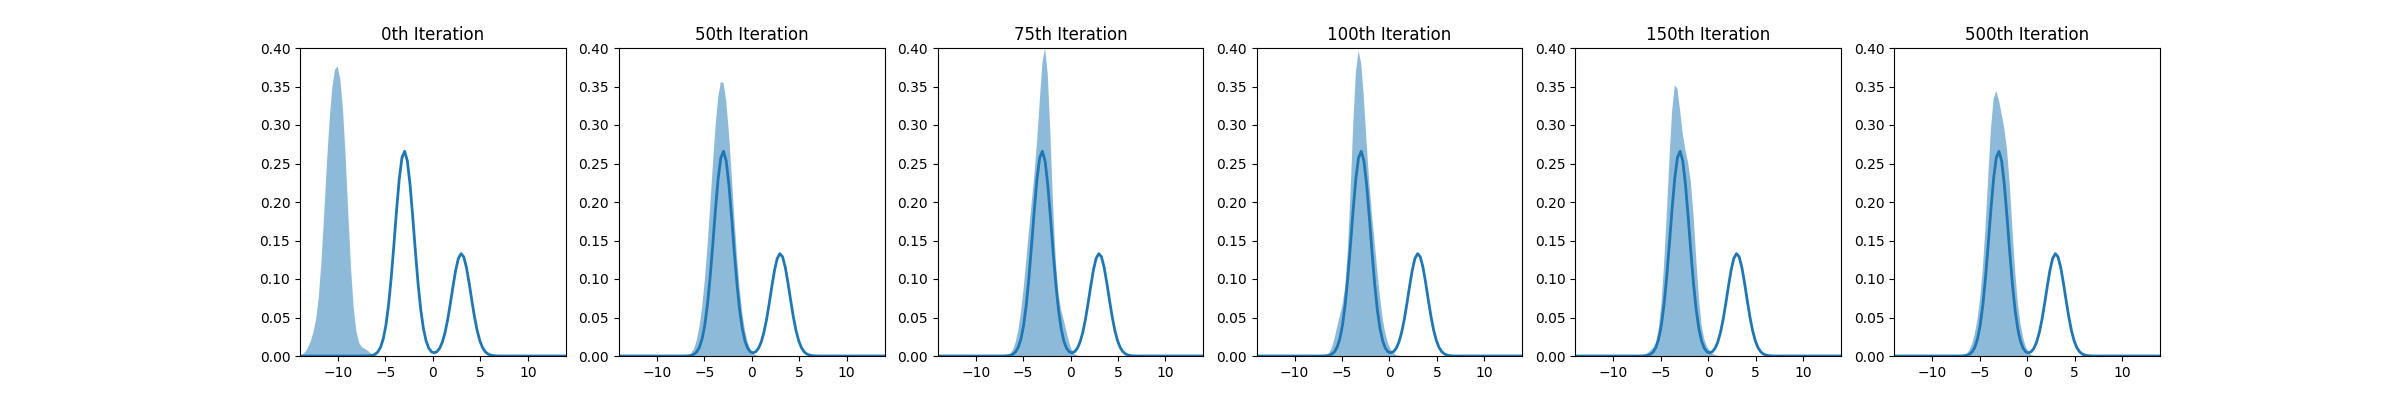
\includegraphics[width=\textwidth]{figs/toy-figure1_step0.25_mu3.0_w0.67_gaussian.png} \\
        \small (4) StepSize = 0.25, $\mu = \pm 3$, $(w_1, w_2) = (0.67, 0.33)$
    \end{tabular}
    
    \begin{tabular}{@{}c@{}}
        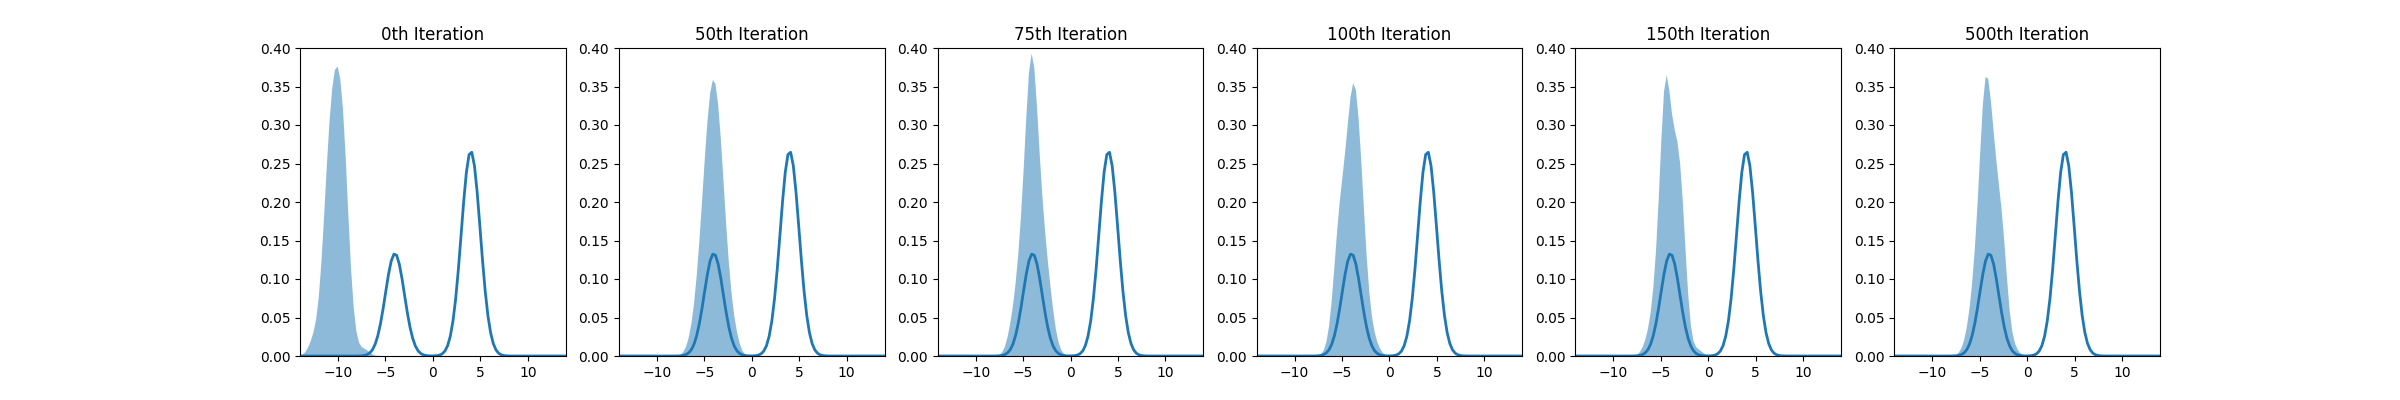
\includegraphics[width=\textwidth]{figs/toy-figure1_step0.25_mu4.0_w0.33_gaussian.png} \\
        \small (5) StepSize = 0.25, $\mu = \pm 4$, $(w_1, w_2) = (0.33, 0.67)$
    \end{tabular}
     
    \caption{Toy example with 1D Gaussian mixture. Particle densities are visualized by KDE.}
    \label{fig:toy1dgaussian}
\end{figure}

\begin{figure}[h]
    \centering
    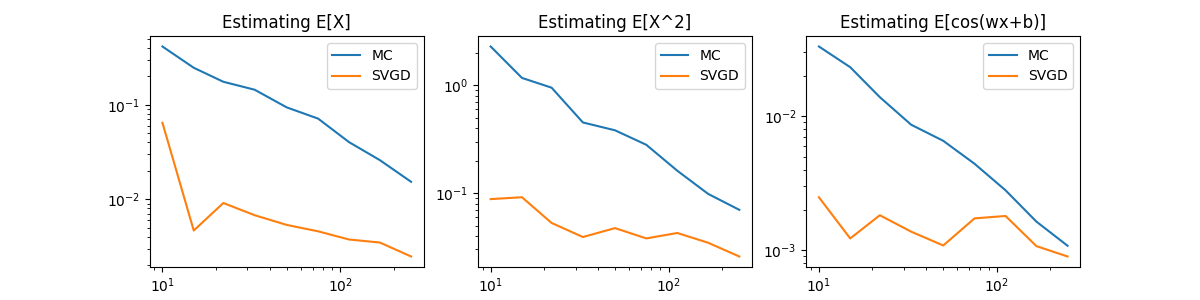
\includegraphics[width=\textwidth]{figs/toy-figure2.png}
    \caption{Comparison between MC and SVGD on simple mean estimation tasks. }
    \label{fig:my_label}
\end{figure}

\subsection{Bayesian Logistic Regression}
\subsubsection{Small scale}
We attempt to test the SVGD algorithm in small-scale logistic regression tasks. We aim to construct a model which is able to predict a binary label of some training data. We run the SVGD algorithm as implemented on NumPyro against the No U-Turn Sampler (NUTS) algorithm. We model the logistic regression problem as a model in NumPyro, and simply perform inference on them but using NUTS and SVGD. The result is shown in Figure \ref{fig:logist_small}.

\subsubsection{Large scale}
We also attempt to compare the performance of SVGD with other optimization algorithms on large scale Bayesian logistic regression in terms of test accuracy with respect to the number of iterations and particle size. We use the same dataset the original paper used, which is the binary Covertype dataset. The dataset contains 581012 data entries and each data point has 54 features. The binary Covertype dataset is a special variant of the original Covertype dataset which has 7 output classes. The binary version combines two output classes out of the 7 into class 1, and treats the rest classes as class 0. This dataset is very large even for current computers. If we do not use stochastic gradient descent and load all data in one batch, we would most likely encounter memory overflow. 

The baseline we choose is stochastic gradient Langevin dynamics (SGLD), where a noise term is added to the gradient in each step. In particular, we use the parallel version of SGLD. 



\begin{figure}[h]
    \centering
    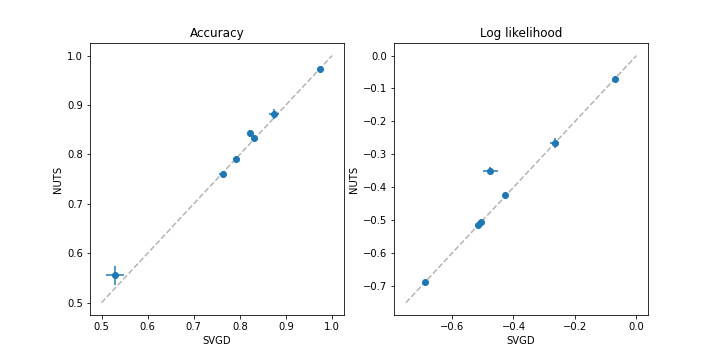
\includegraphics[width=\textwidth]{figs/logistic_svgd_nuts.png}
    \caption{Caption}
    \label{fig:logist_small}
\end{figure}

\subsection{Bayesian Neural Network}

A Bayesian Neural Network (BNN) is a neural network where rather than finding the single optimal value for the model weights, we aim to find a distribution on the model weights that fits with the observations instead.

For the experiments, we train a small BNN on a set of regression tasks. We follow the setup from the paper and use the UCI dataset. We run tests on the SVGD algorithm as implemented by the authors of the original paper and also the implementation on NumPyro, and also on the probabilistic back-propagation (PBP) algorithm. A change that we made was to run each algorithms using the same subsaming size of 100 and ran each algorithms for up to 50 or 200 epochs, depending on the training data size. The other hyperparameters were kept the same as the original code. We report the results in Tables \ref{tab:bnn_rmse} and \ref{tab:bnn_logl}. 

\begin{table}[]
\centering
\caption{Root-mean-squared error (RMSE) on test data for each algorithms} 
\label{tab:bnn_rmse}
\begin{tabular}{|c|ccc|}
\hline
 Dataset & PBP & SVGD (original) & SVGD (NumPyro)  \\
 \hline
boston & $3.007 \pm 0.278$ & $2.987 \pm 0.341$ & $3.290 \pm 0.369$ \\
concrete & $5.435 \pm 0.075$ & $5.240 \pm 0.134$ & $5.567 \pm 0.158$ \\
energy & $1.147 \pm 0.046$ & $0.890 \pm 0.032$ & $1.706 \pm 0.051$ \\
kin8nm & $0.097 \pm 0.001$ & $0.101 \pm 0.001$ & $0.100 \pm 0.001$ \\
naval & $0.006 \pm 0.000$ & $0.004 \pm 0.000$ & $0.003 \pm 0.000$ \\
power & $4.132 \pm 0.046$ & $4.168 \pm 0.053$ & $4.627 \pm 0.055$ \\
protein & $4.668 \pm 0.009$ & $4.493 \pm 0.018$ & $4.655 \pm 0.014$ \\
wine & $0.638 \pm 0.014$ & $0.632 \pm 0.015$ & $0.651 \pm 0.014$ \\
yacht & $0.689 \pm 0.047$ & $3.656 \pm 0.282$ & $3.546 \pm 0.195$ \\
\hline
\end{tabular}
\end{table}

\begin{table}[]
\centering
\caption{Average log-likelihood value on test data for each algorithms} 
\label{tab:bnn_logl}
\begin{tabular}{|c|ccc|}
\hline
 Dataset & PBP & SVGD (original) & SVGD (NumPyro)  \\
 \hline
boston & $-2.879 \pm 0.261$ & $-2.689 \pm 0.158$ & $-2.809 \pm 0.043$ \\
concrete & $-3.150 \pm 0.022$ & $-3.099 \pm 0.032$ & $-3.249 \pm 0.014$ \\
energy & $-1.583 \pm 0.033$ & $-1.309 \pm 0.036$ & $-2.654 \pm 0.004$ \\
kin8nm & $0.913 \pm 0.011$ & $0.871 \pm 0.009$ & $0.793 \pm 0.004$ \\
naval & $3.766 \pm 0.009$ & $3.993 \pm 0.022$ & $4.125 \pm 0.003$ \\
power & $-2.839 \pm 0.011$ & $-2.850 \pm 0.014$ & $-3.219 \pm 0.005$ \\
protein & $-2.960 \pm 0.002$ & $-2.923 \pm 0.005$ & $-2.995 \pm 0.005$ \\
wine & $-0.986 \pm 0.028$ & $-0.968 \pm 0.021$ & $-1.074 \pm 0.033$ \\
yacht & $-1.129 \pm 0.038$ & $-2.741 \pm 0.065$ & $-3.350 \pm 0.004$ \\
\hline
\end{tabular}
\end{table}

In our results, we were able to replicate the superior performance of the SVGD algorithm over the PBP algorithm. In most test cases used, we are able to show that the predictions from the SVGD algorithm is more accurate than that from the PBP algorithm, as measured by the root-mean-squared error of the prediction. 

However, we found that the SVGD algorithm implementation on NumPyro was not able to replicate the performance that the original SVGD algorithm was able to. This could be due to the fact that unlike the SVGD algorithm from the original paper, the SVGD algorithm on NumPyro is minimising the loss based on the ELBO value, and not the true posterior probability. However, to test if this is the 

\begin{figure}[h]
    \centering
    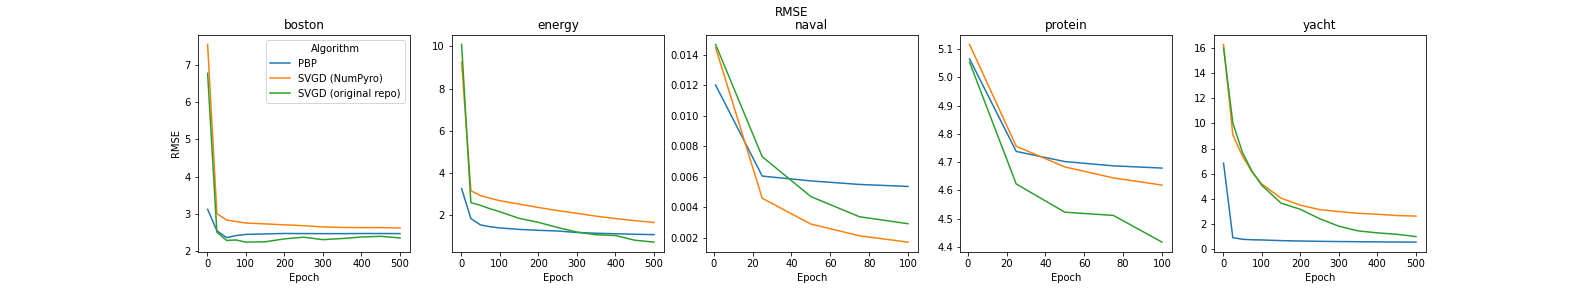
\includegraphics[width=\textwidth]{figs/bayesian_epoch_RMSE.png}
    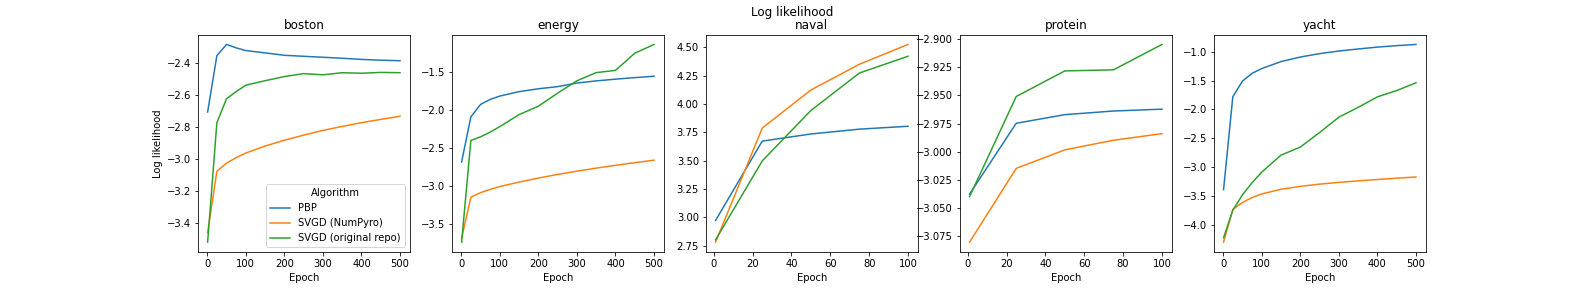
\includegraphics[width=\textwidth]{figs/bayesian_epoch_Loglikelihood.png}
    \caption{Caption}
    \label{fig:my_label}
\end{figure}